\clearpage
\section{移动相机时的光照}
在 Sponza 中庭拉近镜头，观察右边挂毯上方的拱廊。默认的 Lit 视图在移动时保留完整光照。勾选「移动时仅算直接光」后，点光源仍照亮柱面，拱廊下方靠反射光照亮的区域则会变暗。停手约 0.22 秒后，编辑器重新加入 DDGI、GTAO 和 TAA，挂毯背后的暗部开始恢复。

\begin{figure}[H]\centering
\panelimage{.48\linewidth}{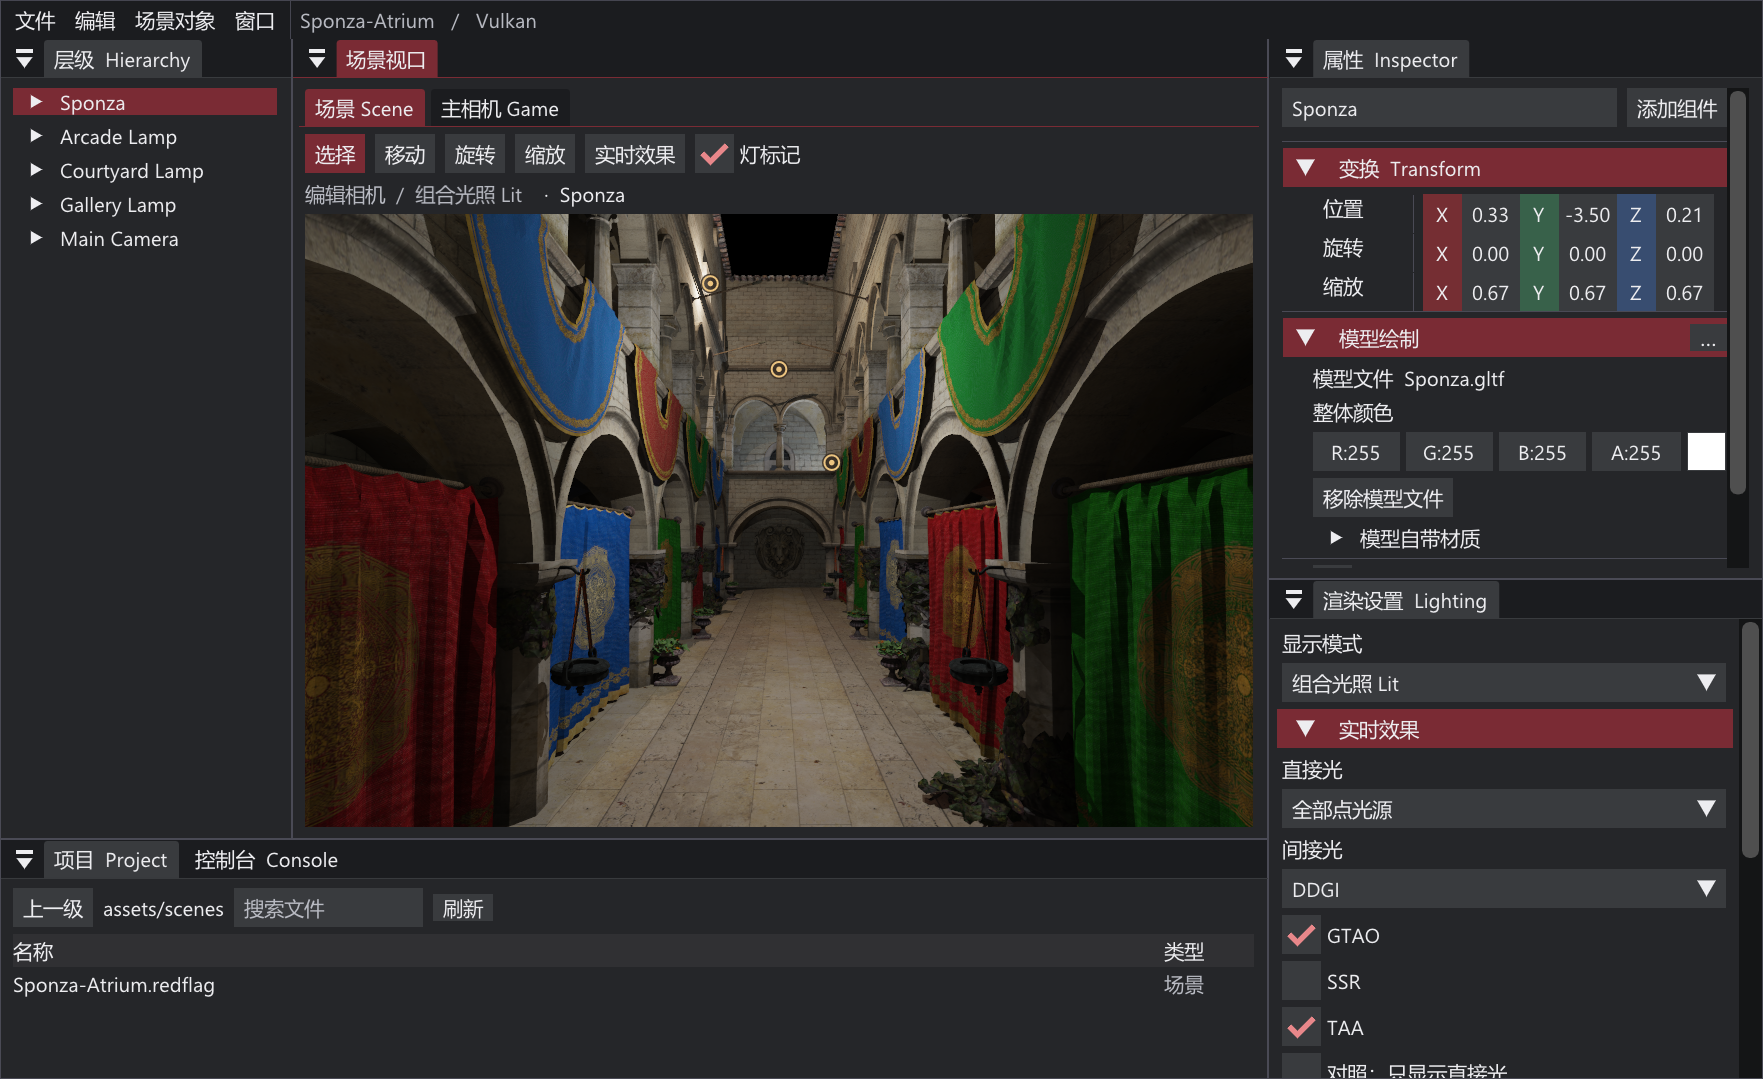
\includegraphics[width=\linewidth,trim=305bp 252bp 510bp 214bp,clip]{navigation-light/lit-motion-move.png}}{默认设置，移动中保留完整光照}
\hfill
\panelimage{.48\linewidth}{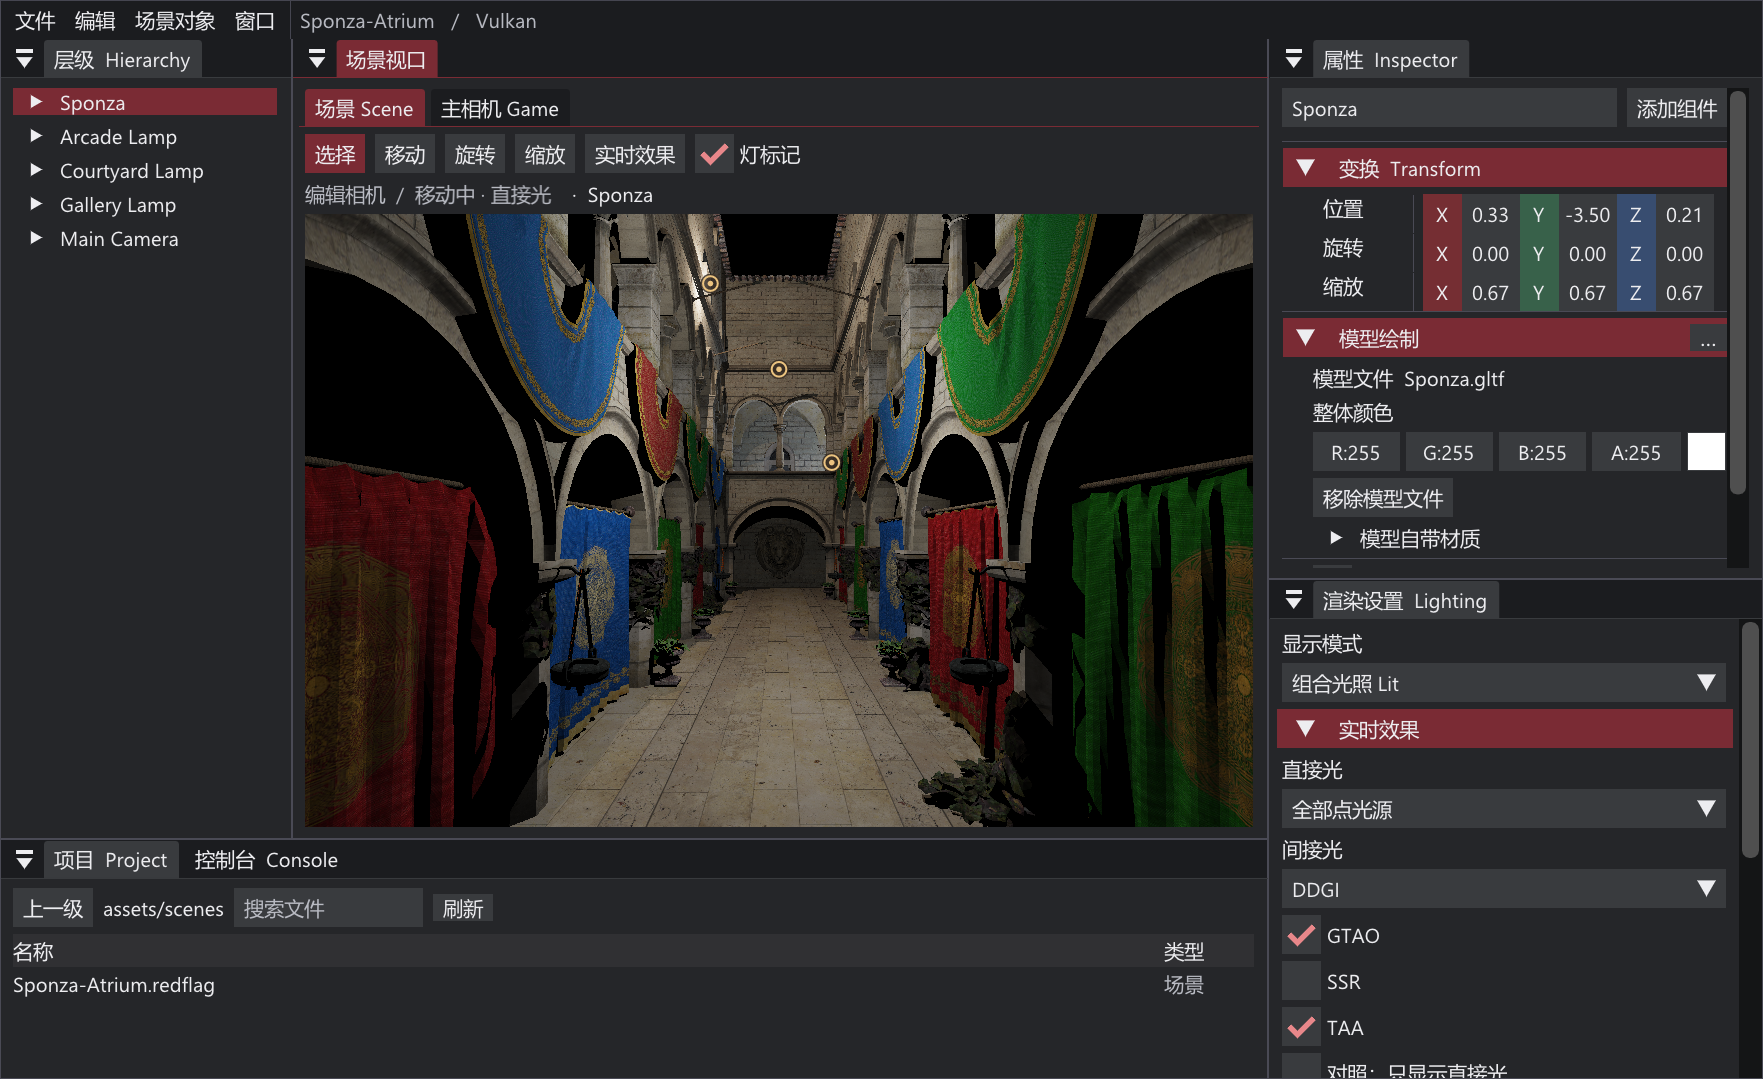
\includegraphics[width=\linewidth,trim=305bp 252bp 510bp 214bp,clip]{navigation-light/navigation-move.png}}{勾选后，同一机位只计算直接光}
\caption{两次均在计时结束后再滚动一格，约 90 毫秒后读取实际窗口，裁出相同的场景面板。两张图里挂毯的纹样和拱门的位置可以逐一对照。}
\end{figure}

关闭其他测试场景后，在同一可执行文件上各运行一次。设备为 RTX 5070 Ti Laptop GPU，Debug x64，Vulkan 验证开启。两轮都是 $948\times613$、三盏点光源、每方向两条射线的 DDGI、GTAO 与历史权重 $0.85$ 的 TAA。每隔 150 毫秒送一次滚轮输入，共 50 次。下表只取新版本中镜头实际改变并重新计算光照的帧，测量整帧经过的时间。两次输入之间直接显示缓存的帧另计。

\begin{center}\smalltable
\begin{tabular}{lrrr}\toprule
镜头改变时显示什么 & 计算帧数 & 中位数（ms） & P95（ms）\\\midrule
保留完整光照 & 50 & 15.24 & 18.62\\
只计算直接光 & 50 & 17.56 & 19.61\\\bottomrule
\end{tabular}
\end{center}

这一轮选用直接光的运动帧反而多用了约 2.3 毫秒。整帧还包含 CPU 调用、等待 GPU 和呈现，两个数不足以把差值归到某个着色器上。两次输入的间隔里，直接光可以复用已有画面。这类缓存帧的中位数是 4.06 毫秒。前页旧版底色导航的 4.15 毫秒覆盖了整个移动时段，当时画的内容和进入统计的帧都不同。

另一次在 RenderDoc 1.47 中边滚动边截取第 39 帧，面板为 $1393\times892$。事件 12 找出相机看到的表面，24 计算点光源直接照明，36 将结果写入供 ImGui 读取的图像。回放中有 103 次场景网格绘制与 22 次界面绘制。截图、事件号与两轮计时见 \path{output/profiling/navigation-light/}。镜头停下后能省去哪些计算，见第~\pageref{perf:baked-still}~页的浴室回放。
